
\chapter{Browser Extensions for Accessibility Audits}
\label{chap:Intro}

Using browser extensions is one way to audit the accessibility of
websites.  This paper evaluates five different extensions for
accessibility auditing: axe DevTools, Accessibility Insights for Web,
Google Lighthouse, Siteimprove and WAVE.  Three of the tools we have
selected for this paper use the \emph{axe-core} library
\parencite{axe_core}, which is an open-source accessibility engine for
automated web UI testing.  As a result, many of the tools will give
similar results and the main difference between the extensions is how
the list of accessibility issues is presented and what additional
features are offered.  The library allows accessibility auditing to
Web Content Accessibility Guidelines (WCAG) 2.0 and 2.1 on the levels
A and AA.

Most of the browser extensions evaluated in this paper are completely free.
Only axe DevTools offers a paid version of the extension with additional features.

\begin{table}[h]
\tablestretch
\rowcolors{2}{}{tablerowcolour}
\centering
\begin{tabularx}{\linewidth}
{>{\kern-\tabcolsep}lllXX<{\kern-\tabcolsep}}
\toprule
\textbf{Extension} & \textbf{Browser} & \textbf{Licence} & \textbf{Downloads\footnotemark}
\\
\midrule
axe DevTools & Chrome, Edge & Free, commercial & 210000 \\
%
Accessibility Insights for Web & Chrome, Edge & Free, open-source & 120000 \\
%
Google Lighthouse & Chrome (built-in) & Free, open-source & 900000\footnotemark \\
%
Siteimprove Accessibility Checker & Chrome, Firefox, Edge, Opera & Free & 30000 \\
%
WAVE Evaluation Tool & Chrome, Firefox, Edge & Free & 520000 \\
\bottomrule
\end{tabularx}
\caption[Browser Extensions Information]
{
Browser extensions information \\
% TODO: Figure out how to use \footnotetext here
\textsuperscript{1}\text{Data collected from Chrome Web Store, Opera Addons, Firefox Add-ons and Microsoft Edge Add-ons.} \\
\textsuperscript{2}\text{Google Lighthouse is built-in into Google Chrome, so the actual number of users may be significantly higher.}
}
\label{tab:browser-extensions-info}
\footnotetext{test}
\end{table}

\section{axe DevTools}
Axe DevTools \parencite{axe_devtools} is a tool for auditing accessibility developed by Deque Systems Inc.
The browser extension is based on the \emph{axe-core} underlying library for auditing the accessibility, but also offers some additional stricter audit rules compared to the base \emph{axe-core} library, allowing validation according to WCAG 2.1 AAA.
The extension is available for Chrome and Edge.
The Deque website contains a link to the axe DevTools extension for Firefox, but at the time of writing this paper it does not seem to work.

There are three different plans available, Free, Pro and Enterprise.
The free version has a limited set of features and mostly consists of only the automated testing of accessibility.
The Pro version costs \$40 per month and offers additional features, such as guided manual tests, partial accessibility testing and exporting of accessibility issues.
Lastly, the Enterprise version of axe DevTools offers even more features, for example CI/CD integration and custom rules.

The descriptions of the accessibility issues are great, but short.
However, links are provided to the Deque accessibility rule documentation for learning more about the accessibility issues and how to fix them.
The element highlighting in the extension is excellent and works better than the highlighting in the rest of the extensions evaluated in this survey.


\begin{figure}[h]
\centering
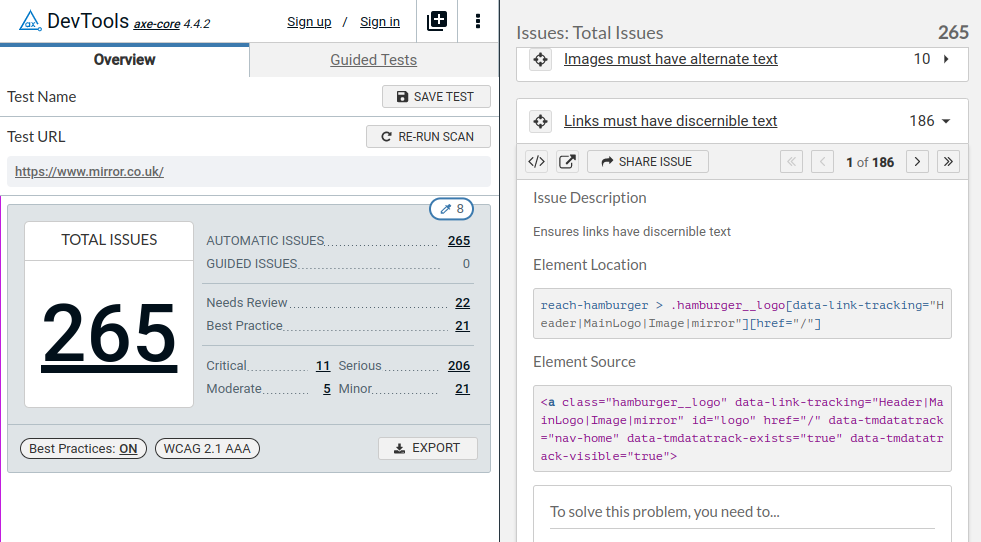
\includegraphics[keepaspectratio,width=\linewidth,height=\halfh]
{images/axe-devtools-ext.png}

\caption[axe DevTools]{
The accessibility of https://mirror.co.uk audited using axe DevTools.
}
\label{fig:axe-devtools-ext}
\end{figure}

\section{Accessibility Insights for Web}
Accessibility Insights for Web \parencite{accessibility_insights} is a browser extension for accessibility auditing using Chrome or Edge.
The extension offers two different audit methods, automated checking, known as FastPass, and manual assessment.
The FastPass automated check provides accessibility auditing using the the axe-core library.
The accessibility issues are then visible in a list and can be exported as an HTML report or directly to GitHub Issues or Azure Boards for easy integration in the development process.
The manual assessment in the browser extension consists of extensive step-by-step instructions for auditing the accessibility manually.
Of the browser extensions evaluated in this paper, Accessibility Insights for Web is the only free tool to offer support for manual testing.

Another feature available in the extension is the visualization of accessibility issues directly on the web page, similar to how WAVE evaluation tool works.
This allows scrolling the web page to see where accessibility issues occur.
The visualization, or highlighting, of the elements on the web page works nicely and the descriptions of the accessibility issues are good too.


\begin{figure}[h]
\centering
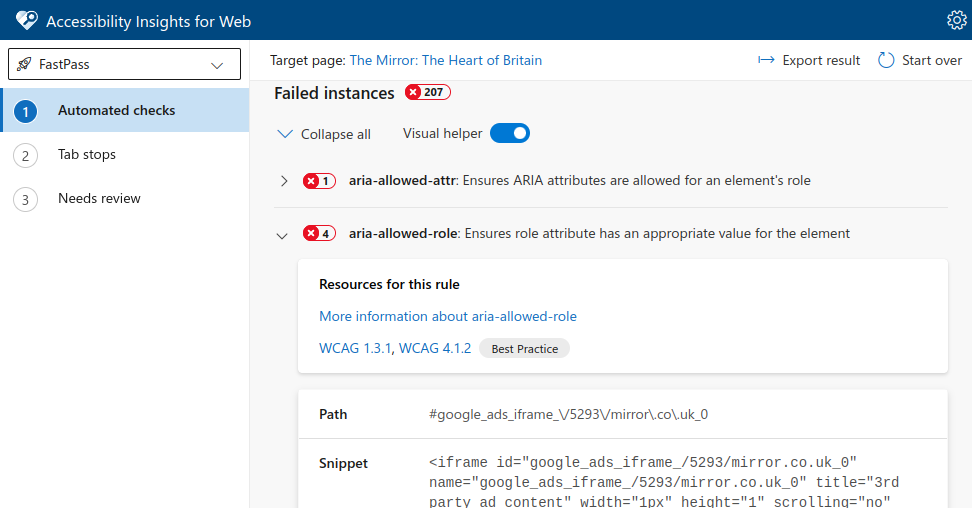
\includegraphics[keepaspectratio,width=\linewidth,height=\halfh]
{images/insights-ext.png}

\caption[Accessibility Insights for Web]{
The accessibility of https://mirror.co.uk audited using Accessibility Insights for Web.
}
\label{fig:insights-ext}
\end{figure}

\section{Google Lighthouse}
Google Lighthouse \parencite{lighthouse} is a the most popular tool for auditing accessibility, which is included in Google Chrome.
Lighthouse, like the previous browser extensions, is also based on the \emph{axe-core} library.
For auditing accessibility, Lighthouse offers a relatively basic set of features, and relies heavily on integration with Chrome DevTools and external references for accessibility issue descriptions.
Accessibility issues are presented as a list of what accessibility checks have passed and which ones have failed.

The descriptions of the issues are decent, and links to the Deque documentation are provided to gain a better understanding of what the issues are and how to fix them.
Highlighting of elements with accessibility issues in Lighthouse is not as good as in the other tools.
In many cases the either the link to the code for the element, or the scrolling to the element do not work.
The accessibility audit report can be exported as JSON.
Overall, the extension provides a decent set of features, and is very convenient to use as it is built-in into Chrome.
However, many of the other extension provide nicer presentation of the accessibility issues.


\begin{figure}[h]
\centering
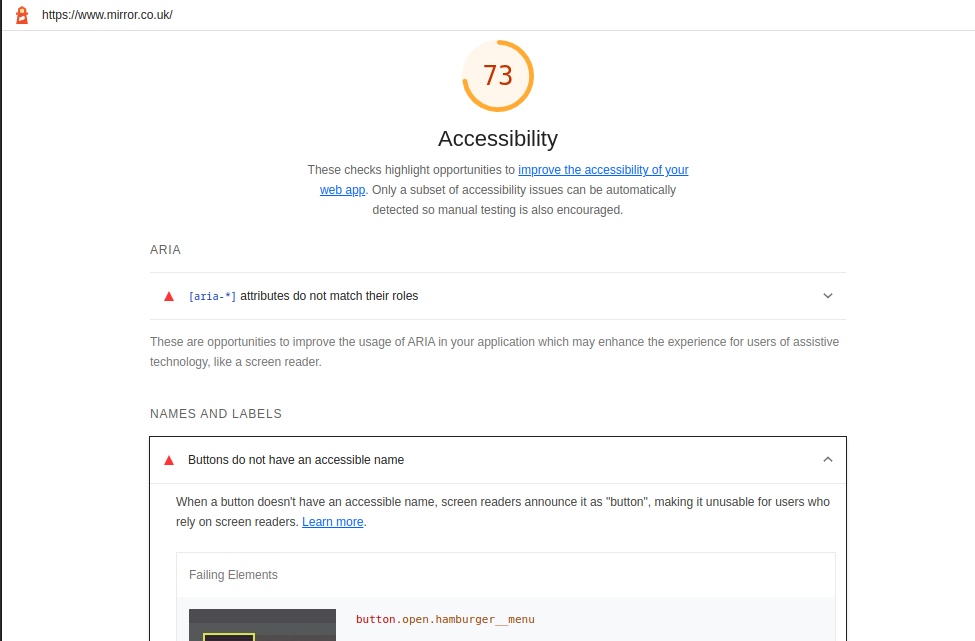
\includegraphics[keepaspectratio,width=\linewidth,height=\halfh]
{images/lighthouse-ext.png}

\caption[Google Lighthouse]{
The accessibility of https://mirror.co.uk audited using Google Lighthouse.
}
\label{fig:lighthouse-ext}
\end{figure}

\section{Siteimprove Accessibility Checker}
Siteimprove Accessibility Checker \parencite{siteimprove} is the least used accessibility audit browser extension out of the extensions in this survey.
The extension presents the accessibility issues as a list, where you can expand each issue to read the description of it and highlight the element on the web page.
Some features that the extension offers, that the other extensions do not offer is simulation of color blindness and excellent filtering of accessibility issues.
The list of issues can also be filtered by difficulty, role, WCAG level and HTML element type.

Descriptions of the accessibility issues found by the extension are quite short, but links to additional descriptions are provided.
The extension also provides code examples for examples on how to fix the accessibility issues, but the usefulness of these examples is limited as the example code can not always be applied in real world scenarios.
Overall, the extension provides a good set of features for auditing the accessibility.
However, one feature that is not offered, which is offered by other tools, is the possibility of exporting the audit report.

\begin{figure}[h]
\centering
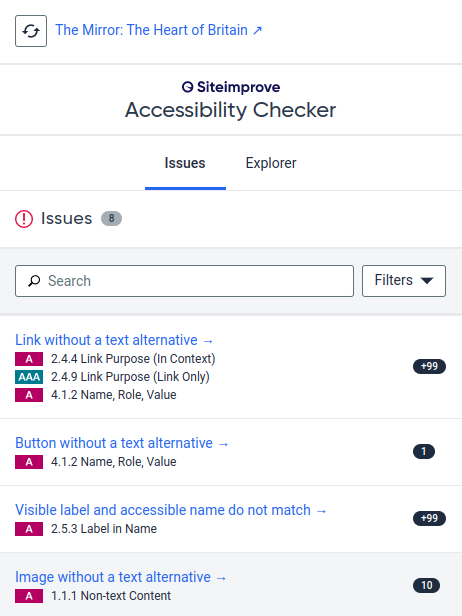
\includegraphics[keepaspectratio,width=\linewidth,height=\halfh]
{images/siteimprove-ext.png}

\caption[Siteimprove Accessibility Checker]{
The accessibility of https://mirror.co.uk audited using Siteimprove Accessibility Checker.
}
\label{fig:siteimprove-ext}
\end{figure}

\section{WAVE Evaluation Tool}
The WAVE evaluation tool \parencite{wave} is another extension for auditing accessibility, supporting Chrome, Firefox and Edge.
The extension functions somewhat differently than the other extensions, as the tool is embedded directly on the web page.
It then inserts icons for elements that fail or succeed in the accessibility checks.
The user can then scroll the web page and click the icons to learn more about the accessibility issue.
Descriptions of the accessibility issues in the built-in reference are decent and links are provided for further information.
As the tool is very interactive, the element highlighting is a fundamental part of the extension, which also works well.

Some special features that WAVE offers are the evaluation of page structure and a tool for contrast checking.
The extension does not offer exporting of the audit report, which is acceptable considering that the tool relies on scrolling the web page to find the accessibility issues.
Elements with accessibility issues are somewhat difficult to find in the code in the extension, as the extension uses its own code browser, which can not be resized at all.

\begin{figure}[h]
\centering
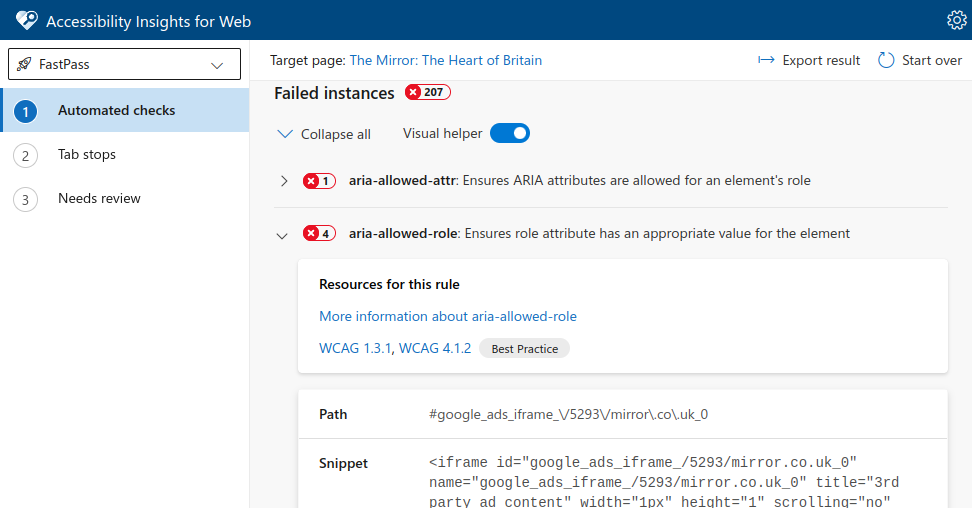
\includegraphics[keepaspectratio,width=\linewidth,height=\halfh]
{images/insights-ext.png}

\caption[WAVE Evaluation Tool]{
The accessibility of https://mirror.co.uk audited using WAVE Evaluation Tool.
}
\label{fig:wave-ext}
\end{figure}


\section{Showcase videos}
For each of the browser extension, we have recorded videos to showcase the extension and their features.
Using each extension, we performed an accessibility audit of http://www.gov.uk/ http://www.mirror.co.uk/.
The showcase videos for axe DevTools \parencite{axe_ext_vid}, Accessibility Insights for Web \parencite{aiweb_ext_vid}, Google Lighthouse \parencite{lighthouse_ext_vid}, Siteimprove Accessibility Checker \parencite{siteimprove_ext_vid}, WAVE Evaluation tool are available online \parencite{wave_ext_vid}.

\section{Browser Extensions Conclusion}
There are many good browser extensions for auditing accessibility of web pages, and all of the extensions evaluated in this survey would be good options for auditing accessibility.
Which extension is the most suitable one depends on what features are needed, what accessibility issues are the most important ones to audit on the web page, what WCAG level is required, and the budget.
For overall accessibility auditing with good descriptions and element highlighting that works well, axe DevTools, Accessibility Insights for Web and Siteimprove are excellent choices.
If a WCAG level of AAA is required, the only suitable extensions are axe DevTools and Siteimprove as the rest of the extensions do not audit as strictly.

